Clusteralgorithmen wirken dem Problem hoher Autokorrelationszeiten im Bereich des Phasenübergangs entgegen.\\
Um dies zu erreichen arbeiten sie nicht mehr nur Lokal, wie der Metropolis Algorithmus, sondern bilden größere Bereiche (Cluster), die auf einmal manipuliert werden.

\subsection{Wolff-Algorithmus}
Der Wolff-Algorithmus ist ein Cluster-Algorithmus, der pro Monte-Carlo-Schritt von einem zufälligen Startpunkt aus ein Cluster bildet und dann mit einer bestimmten Wahrscheinlichkeit alle Spins innerhalb des Clusters flippt.\\\\
Allgemeiner Programmablauf:\\
1. Startkonfiguration (Abbildung \ref{cu2veransch}a)\\
2. Bestimmte einen zufälligen Startpunkt (Abbildung \ref{cu2veransch}b)\\
3. Ausgehend vom Startpunkt werden benachbarte Atome mit gleichem Spin mit Wahrscheinlichkeit p in den Cluster aufgenommen (Abbildung \ref{cu2veransch}c,d,e)\\
4. Flippe alle Spins des Clusters mit einer Wahrscheinlichkeit (Abbildung \ref{cu2veransch}f)\\
5. Gehe zu 1.\\
\begin{figure}[H]
	\centering
	\subfigure[]{
		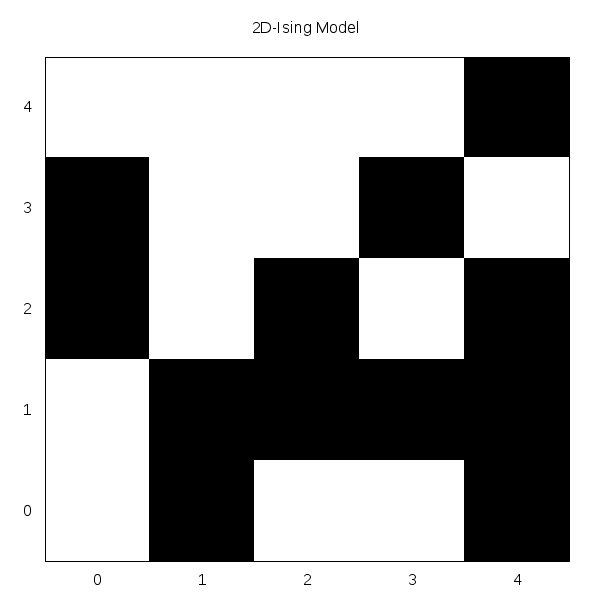
\includegraphics[width=0.25\textwidth]{../Graph_Export/cluster_veranschaulichung/Abbildung41.png}
	}
	\subfigure[]{
		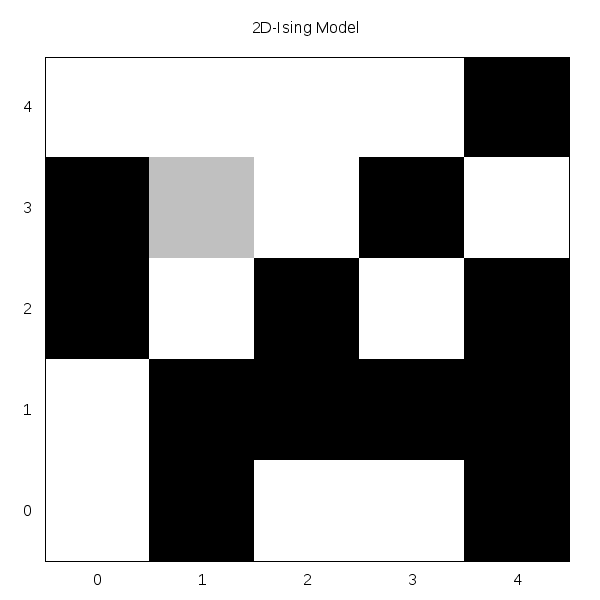
\includegraphics[width=0.25\textwidth]{../Graph_Export/cluster_veranschaulichung/Abbildung42.png}
	}
	\subfigure[]{
		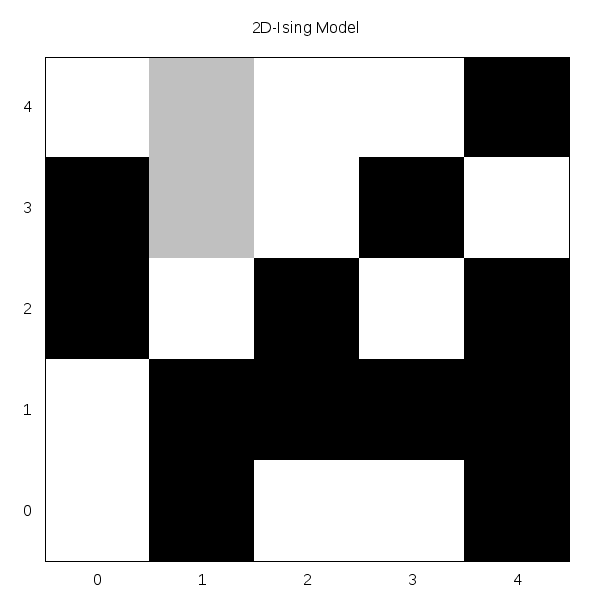
\includegraphics[width=0.25\textwidth]{../Graph_Export/cluster_veranschaulichung/Abbildung43a.png}
	}
	\subfigure[]{
		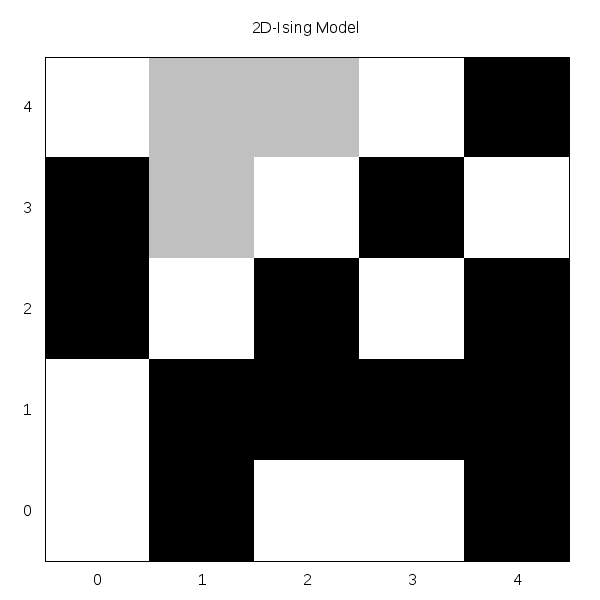
\includegraphics[width=0.25\textwidth]{../Graph_Export/cluster_veranschaulichung/Abbildung43b.png}
	}
	\subfigure[]{
		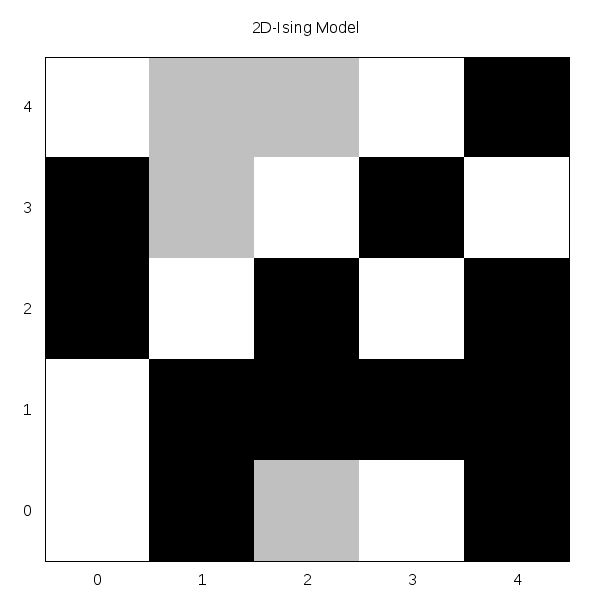
\includegraphics[width=0.25\textwidth]{../Graph_Export/cluster_veranschaulichung/Abbildung43c.png}
	}
	\subfigure[]{
		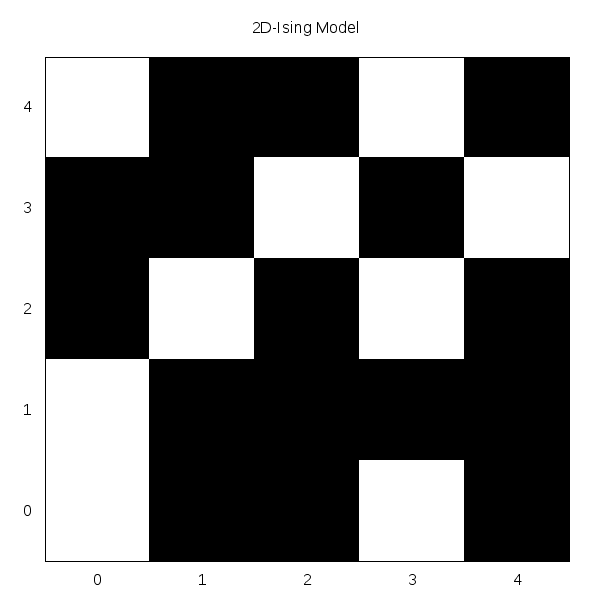
\includegraphics[width=0.25\textwidth]{../Graph_Export/cluster_veranschaulichung/Abbildung44.png}
	}
	\caption{Veranschaulichung des Wolff-Algorithmus Schemas}
	\label{cu2veransch}
\end{figure}


\subsection{Flipp-Wahrscheinlichkeit des Clusters = 1}
Der Algorithmus wird besonders effizient, da bei einer bestimmten Annahme-Wahrscheinlichkeit p, dass ein Zustand in den Cluster aufgenommen wird, der Cluster in jedem Monte-Carlo-Schritt geflippt wird.\\\\
Warum dies so ist wird klar, wenn man sich die Wahrscheinlichkeit $W_{ij}$ für den Übergang von der Konfiguration i zu j berechnet.
\begin{align}
W_{ij} = min\{1, \frac{A(j \rightarrow i) * P_j}{A(i \rightarrow j) * P_i} \} = min\{1, \frac{A(j \rightarrow i) * e^{-\beta E_j}}{A(i \rightarrow j) * e^{-\beta E_i}} \}
\end{align}
Für die Wahrscheinlichkeit $A(i \rightarrow j)$ den Übergang von i nach j zu betrachten und für die Energie $E_i$ im Zustand i gelten:\\
(Hierbei bedeutet $_{innen}$ jeweils innerhalb und $_{außen}$ außerhalb des Clusters\\
und $n_{gleich}$ bzw. $n_{diff}$ sind die Anzahl Spins, die am Rand gleich bzw. ungleich zu dem Spin innerhalb des Clusters sind.)
\begin{align}
A(i \rightarrow j)=A_{innen} * (1 - p)^{n_{gleich}}\\
A_{innen} = p^{n_{innen}-1} + Z\\
E_i = E_{innen} + E_{außen} - n_{gleich} * J + n_{diff} * J\\
\end{align}
Mit Z der Wahrscheinlichkeit einen Spin im Cluster als Startpunkt gewählt zu haben.\\
Ebenso gilt:
\begin{align}
A(j \rightarrow i)=A_{innen} * (1 - p)^{n_{diff}}\\
E_j = E_{innen} + E_{außen} + n_{gleich} * J - n_{diff} * J\\
\end{align}
Damit gilt:
\begin{align}
W_{ij} &= min\{1, \frac{A_{innen}*(1-p)^{n_{diff}}}{A_{innen}*(1-p)^{n_{gleich}}} * \frac{e^{-\beta E_{innen} + E_{außen} + n_{gleich} * J - n_{diff} * J}}{e^{-\beta E_{innen} + E_{außen} - n_{gleich} * J + n_{diff} * J}}\} \\
&= min\{1, \frac{(1-p)^{n_{diff}}}{(1-p)^{n_{gleich}}} * \frac{e^{-\beta n_{gleich} * J} * e^{+\beta n_{diff} * J}}{e^{+\beta n_{gleich} * J} * e^{-\beta n_{diff} * J}}\}\\
&= min\{1, \frac{(1-p)^{n_{diff}}}{(1-p)^{n_{gleich}}} * \frac{e^{-2\beta n_{gleich} * J}}{e^{-2\beta n_{diff} * J}}\}\\
&= min\{1, \left(\frac{(1-p)}{e^{-2\beta J}}\right)^{n_{diff}} * \left(\frac{e^{-2\beta J}}{(1-p)}\right)^{n_{gleich}}\}
\end{align}
Hieraus lässt sich nun erkennen, dass die Wahrscheinlichkeit vom Zustand i zu j überzugehen gleich $1$ wird, wenn wir $p = 1 - e^{-2\beta J}$ wählen.

\subsection{Metropolis und Cluster-Update im Vergleich}
Der Vorteil des Cluster-Algorithmus ist die schnelle Konverenzgeschwindigkeit in der Nähe des Phasenübergangs bzw. der kritischen Temperatur.\\\\

\begin{figure}[H]
	\centering
	\subfigure[Konvergenz beim Cluster-Update-Verfahren]{
		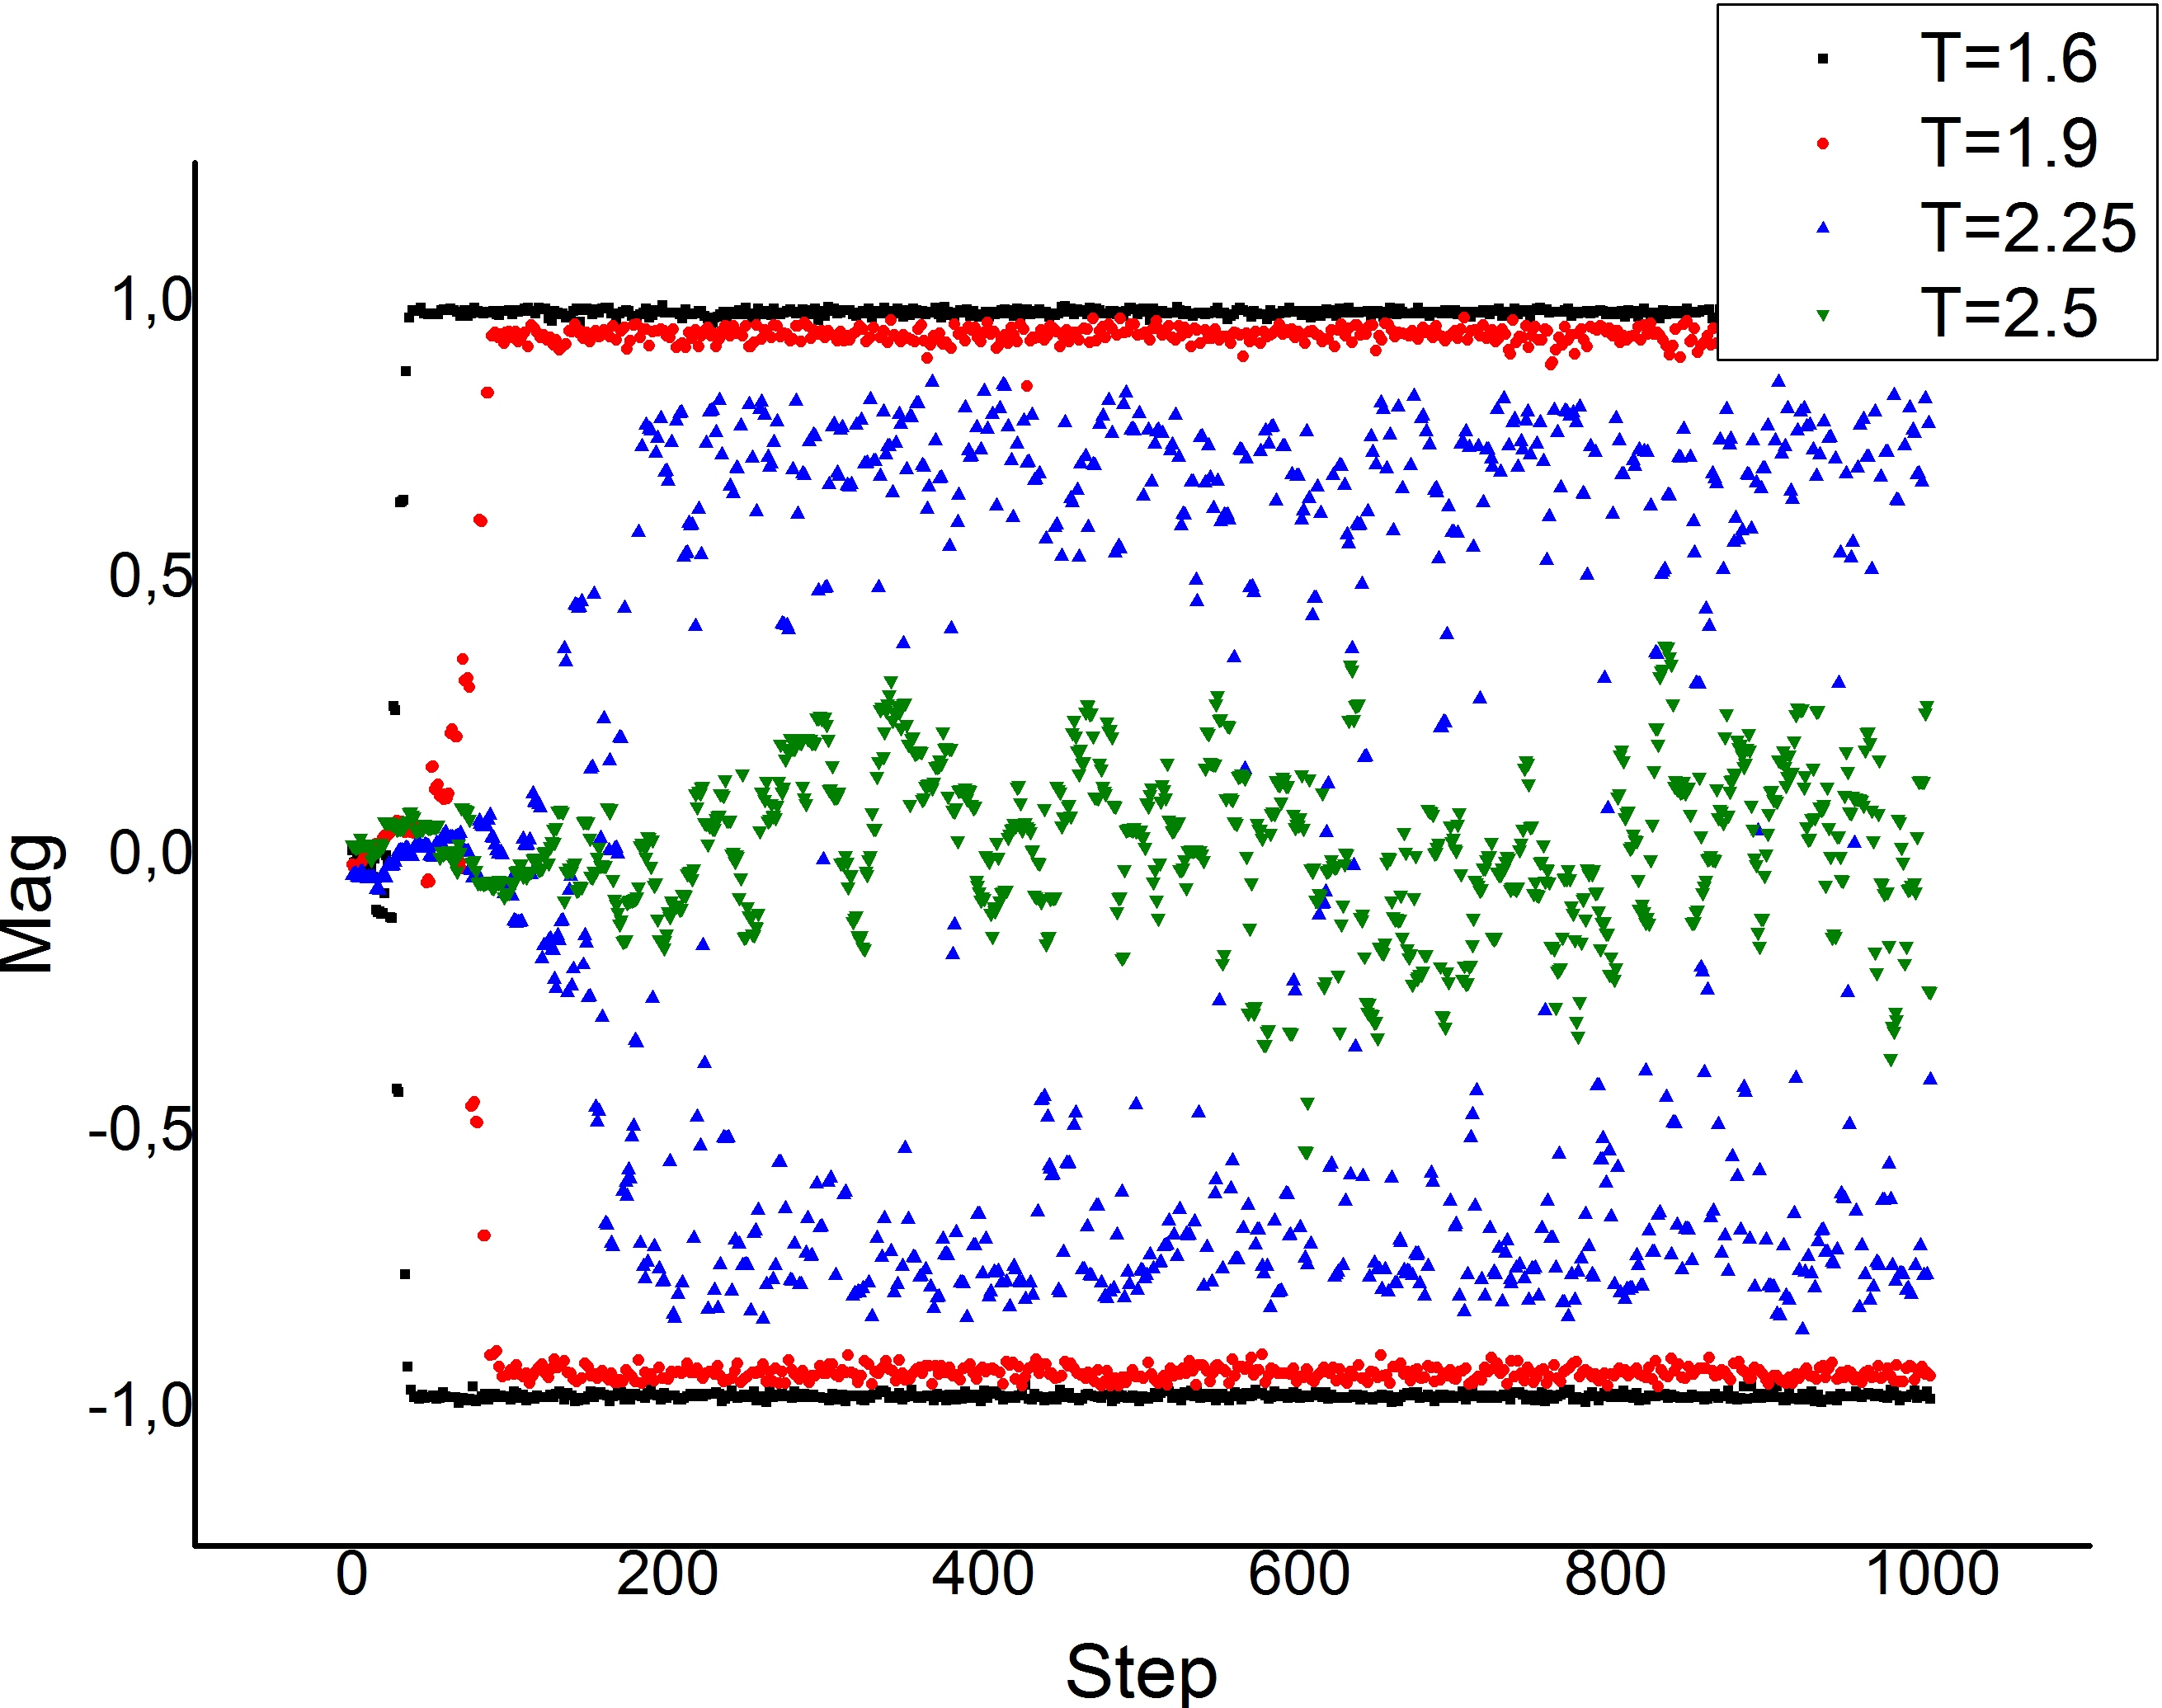
\includegraphics[width=0.30\textwidth]{../Graph_Export/CU2D/m(steps)_Plot.jpg}
	}
	\subfigure[Betragswerte der Abbildung (a)]{
		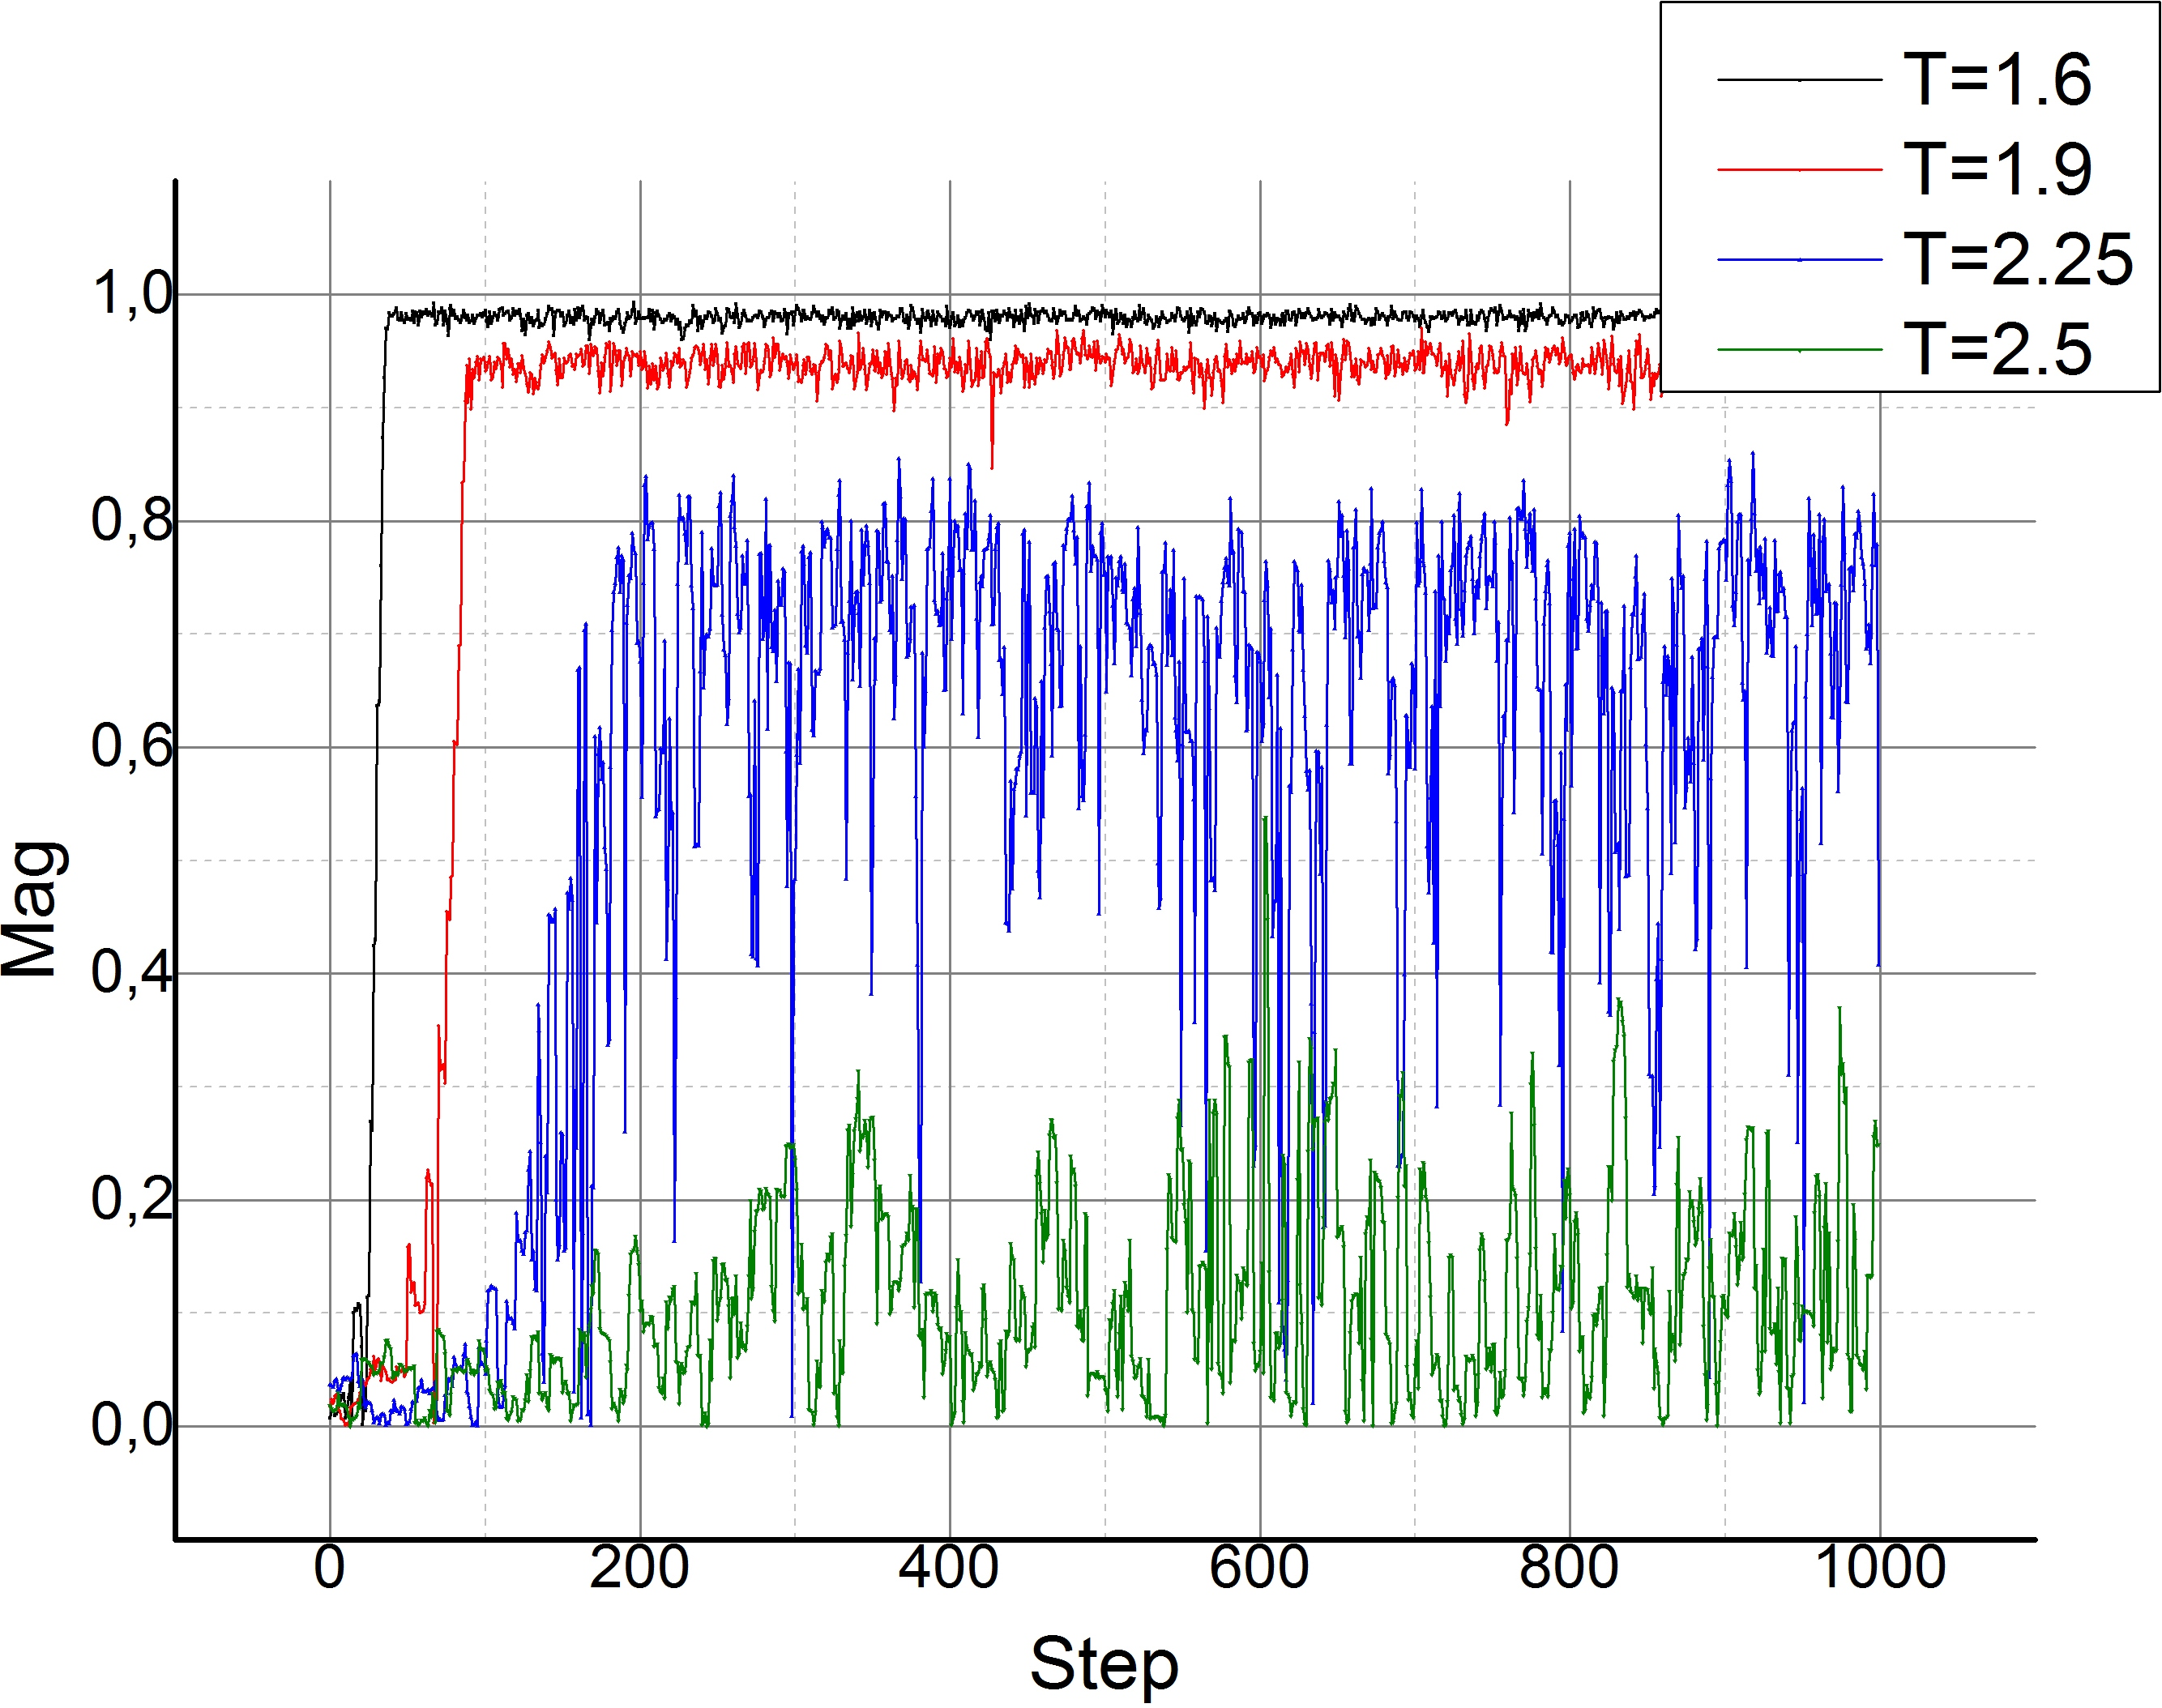
\includegraphics[width=0.30\textwidth]{../Graph_Export/CU2D/abs(m(steps))_Plot.jpg}
	}	
	\subfigure[Konvergenz beim Metropolis-Verfahren]{
		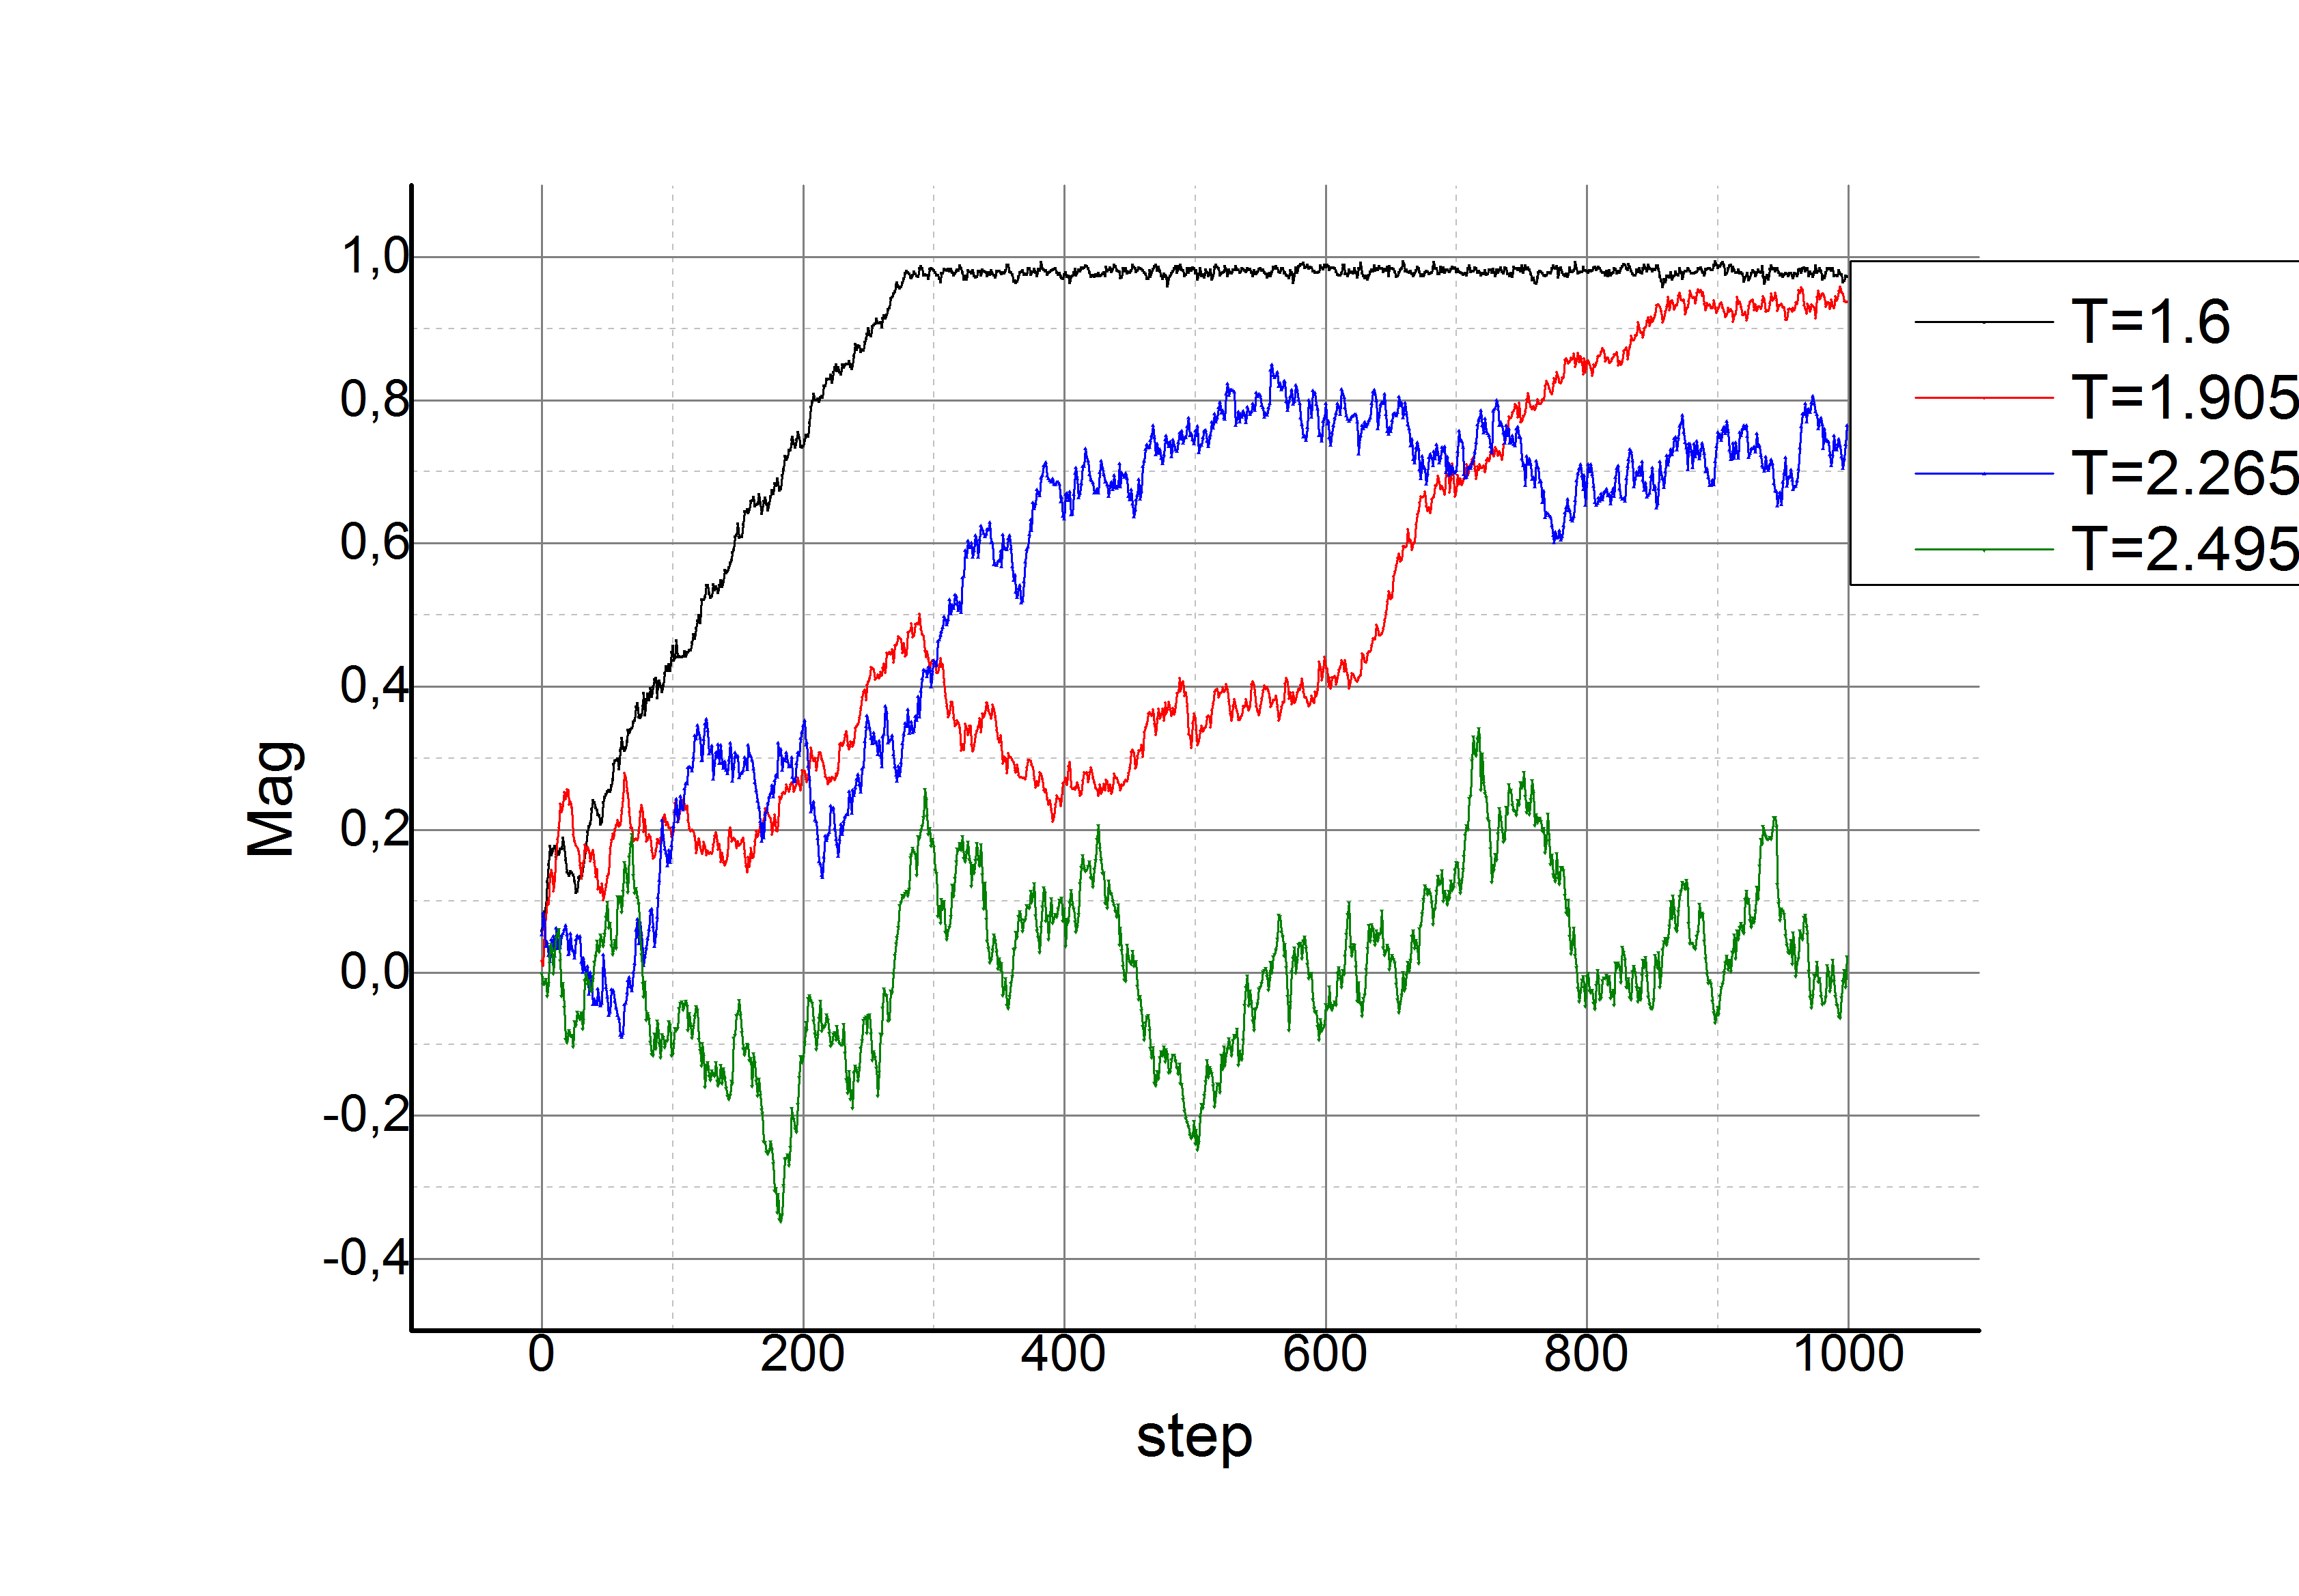
\includegraphics[width=0.30\textwidth]{../Graph_Export/MP2D/m(Steps)_r.jpg}
	}		
	\caption{Konvergenz der Magnetisierung im Vergleich zwischen Metropolis- und Cluster-Update-Verfahren auf einem 50x50 Gitter}
	\label{cu2d2steps}
\end{figure}

Wir erkennen zunächst in Abbildung \ref{cu2d2steps}a, dass es nur Sinn macht, die Betragswerte der Magnetisierung zu betrachten, wenn das Cluster-Update-Verfahren untersucht werden soll. Denn durch das Flippen größerer Cluster springt die Magnetisierung immerzu zwischen negativen und positiven werden.\\
Zu vergleichen sind also sinnvollerweise die Abbildungen \ref{cu2d2steps}b und \ref{cu2d2steps}c. Zunächst ist zu erkennen, dass die Graphen gleicher Temperatur auch gegen die selben Werte konvergieren. Ebenso ist die schnellere Konvergenz des Cluster-Update-Verfahrens deutlich, insbesondere beim Graphen zu $T=1.9$ ist dies schön zu erkennen. Während der Wert beim Metropolis erst nach 800 Schritten gegen 1 konvergiert, tut er dies beim Cluster-Update bereits nach etwa 100. Insofern scheint das Verfahren zu arbeiten, wie erwünscht. Allerdings erzeugt das Cluster-Update sehr stark schwankende Werte für Temperaturen  nahe an Tc oder leicht darüber. Dies liegt wohl daran, dass das Cluster-Update-Verfahren die Instabilität des Systems, die bei diesen Temperaturen vorliegt, stark verdeutlicht, da es global agiert.

\begin{figure}[H]
	\centering
	\subfigure[Konvergenz beim Cluster-Update-Verfahren]{
		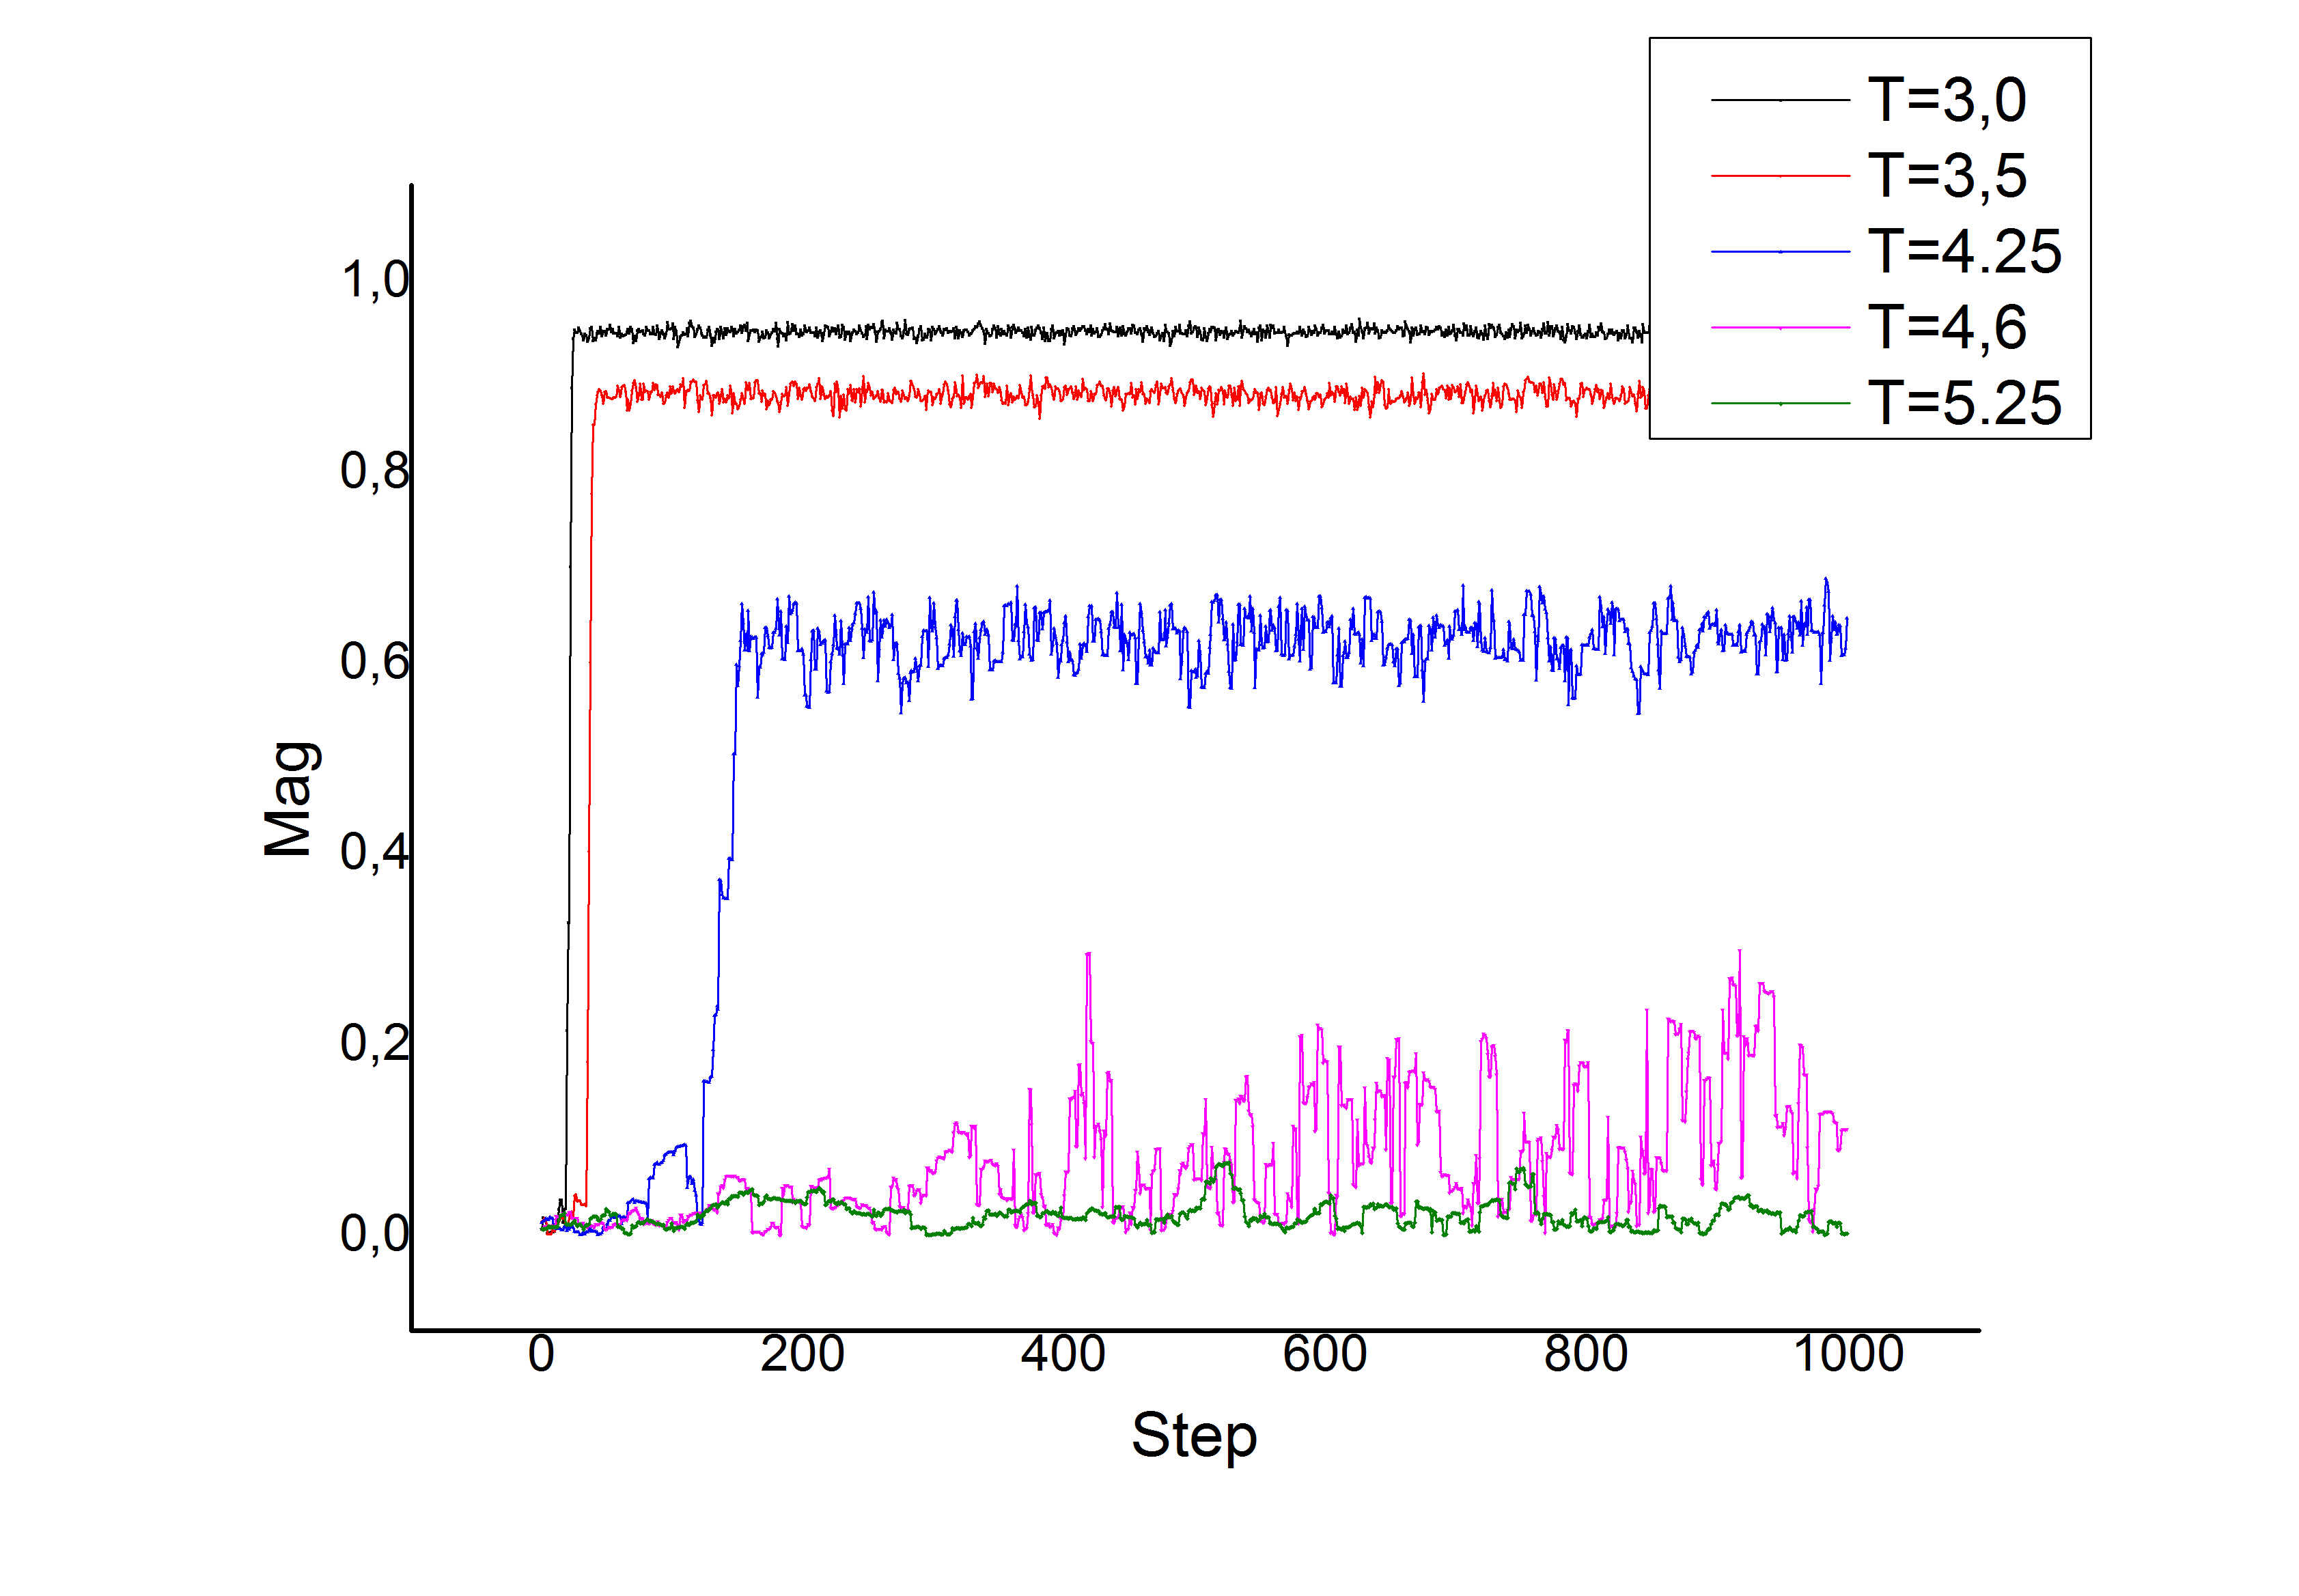
\includegraphics[width=0.47\textwidth]{../Graph_Export/CU3D/abs(m(steps))_Plot.jpg}
	}	
	\subfigure[Konvergenz beim Metropolis-Verfahren]{
		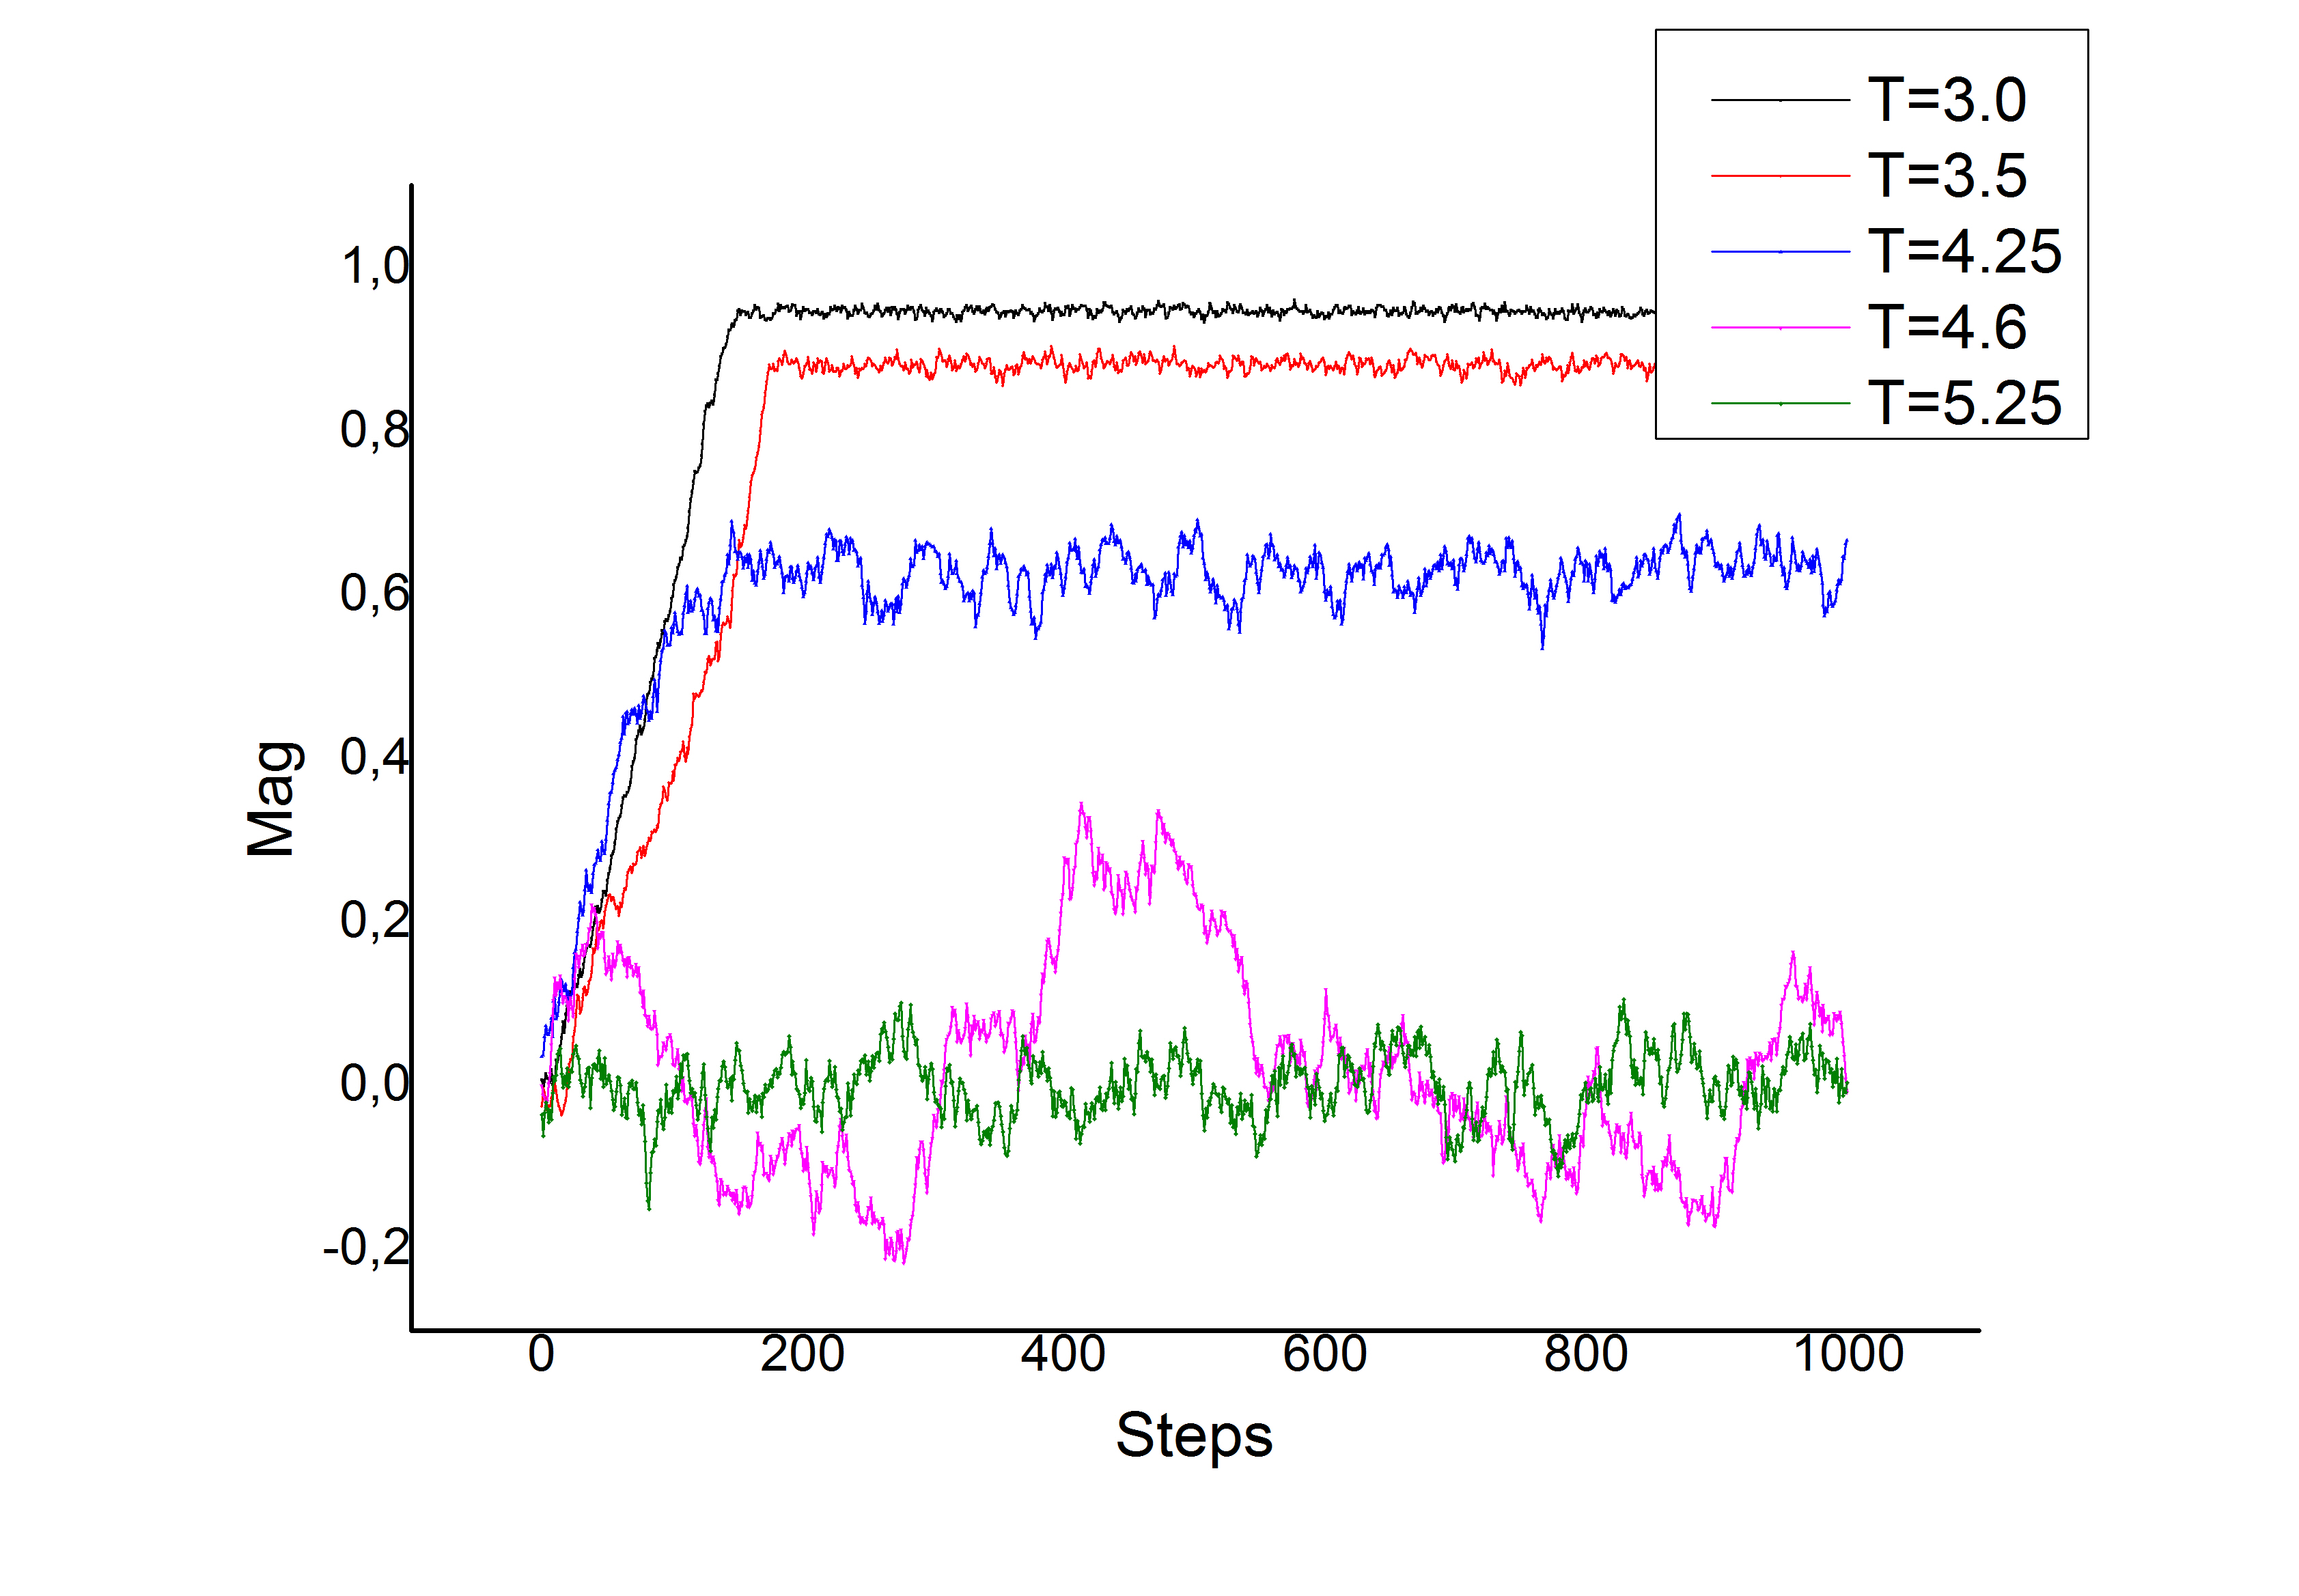
\includegraphics[width=0.47\textwidth]{../Graph_Export/MP3D/m(Steps)_r.jpg}
	}		
	\caption{Konvergenz der Magnetisierung im Vergleich zwischen Metropolis- und Cluster-Update-Verfahren auf einem 20x20x20 Gitter}
	\label{cu2d3steps}
\end{figure}

Bei der Simulation auf einem dreidimensionalen Gitter erkennt man die gleichen Phänomene, wie beim Zweidimensionalen. Die Konvergenz ist insgesamt etwas schneller.

\begin{figure}[H]
	\centering
	\subfigure[Cluster-Update-Verfahren]{
		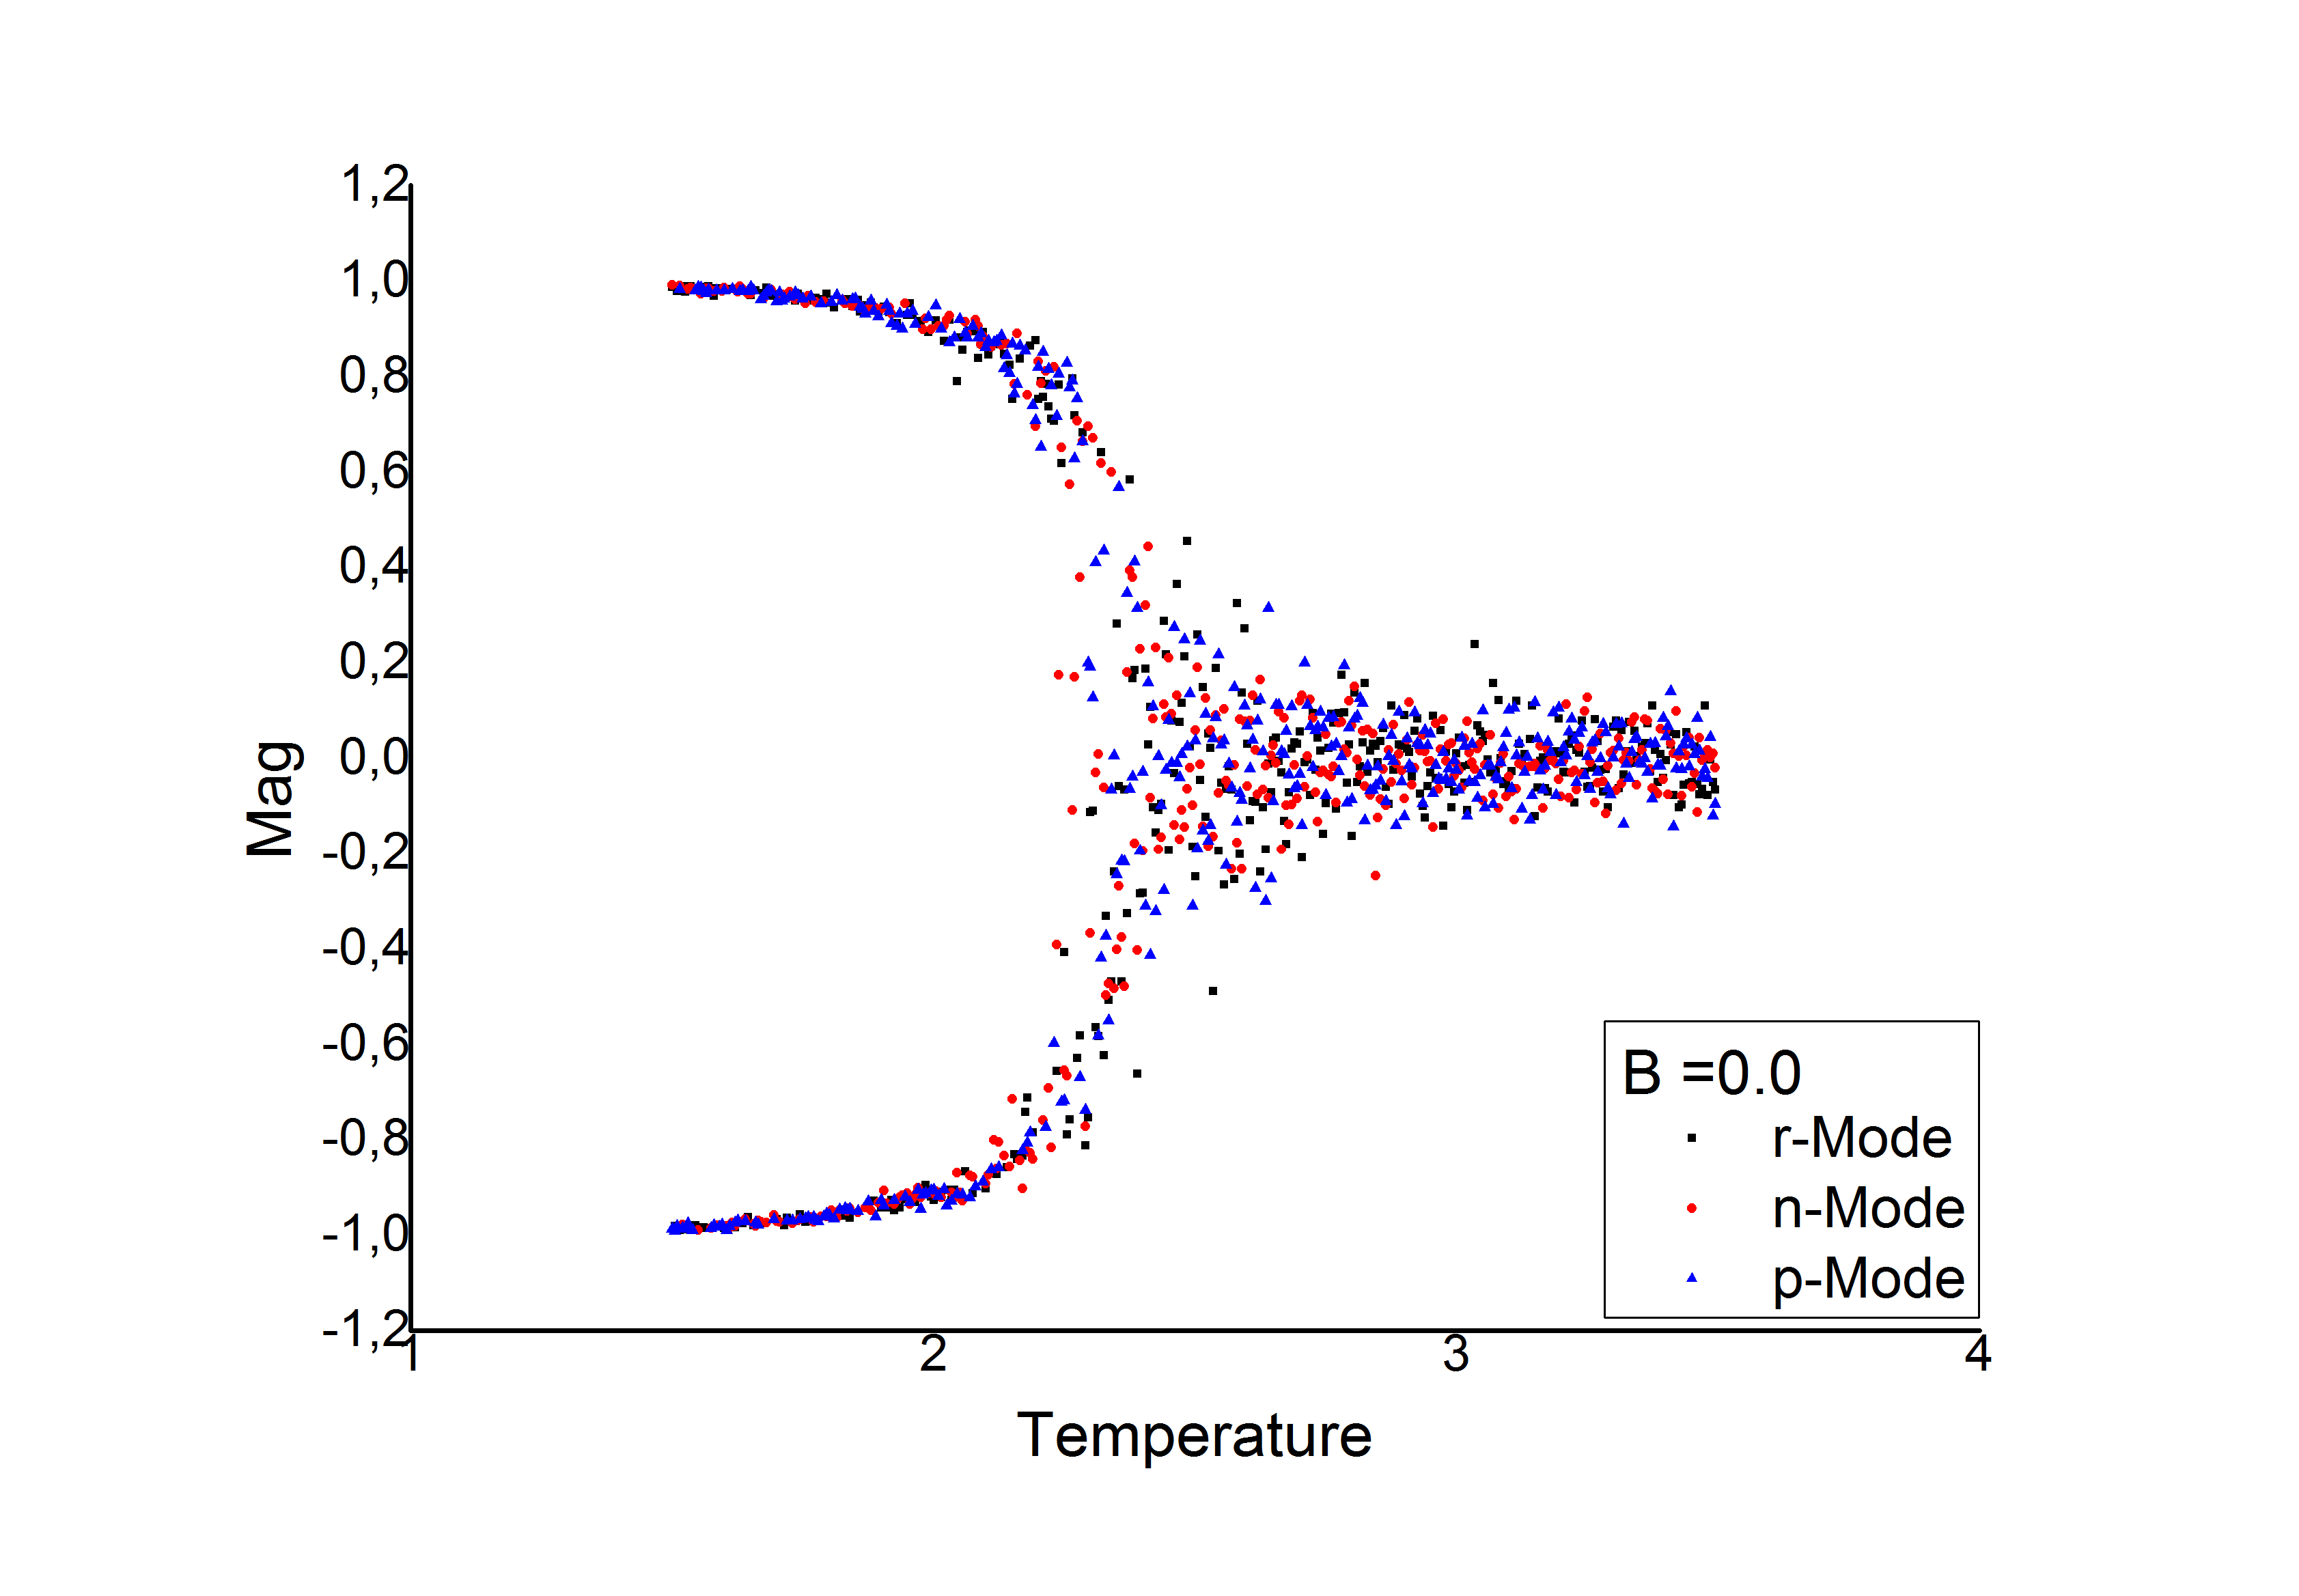
\includegraphics[width=0.47\textwidth]{../Graph_Export/CU2D/m(T)_B=0_matModes_CU2D_Plot.jpg}
	}
	\subfigure[Metropolis-Verfahren]{
		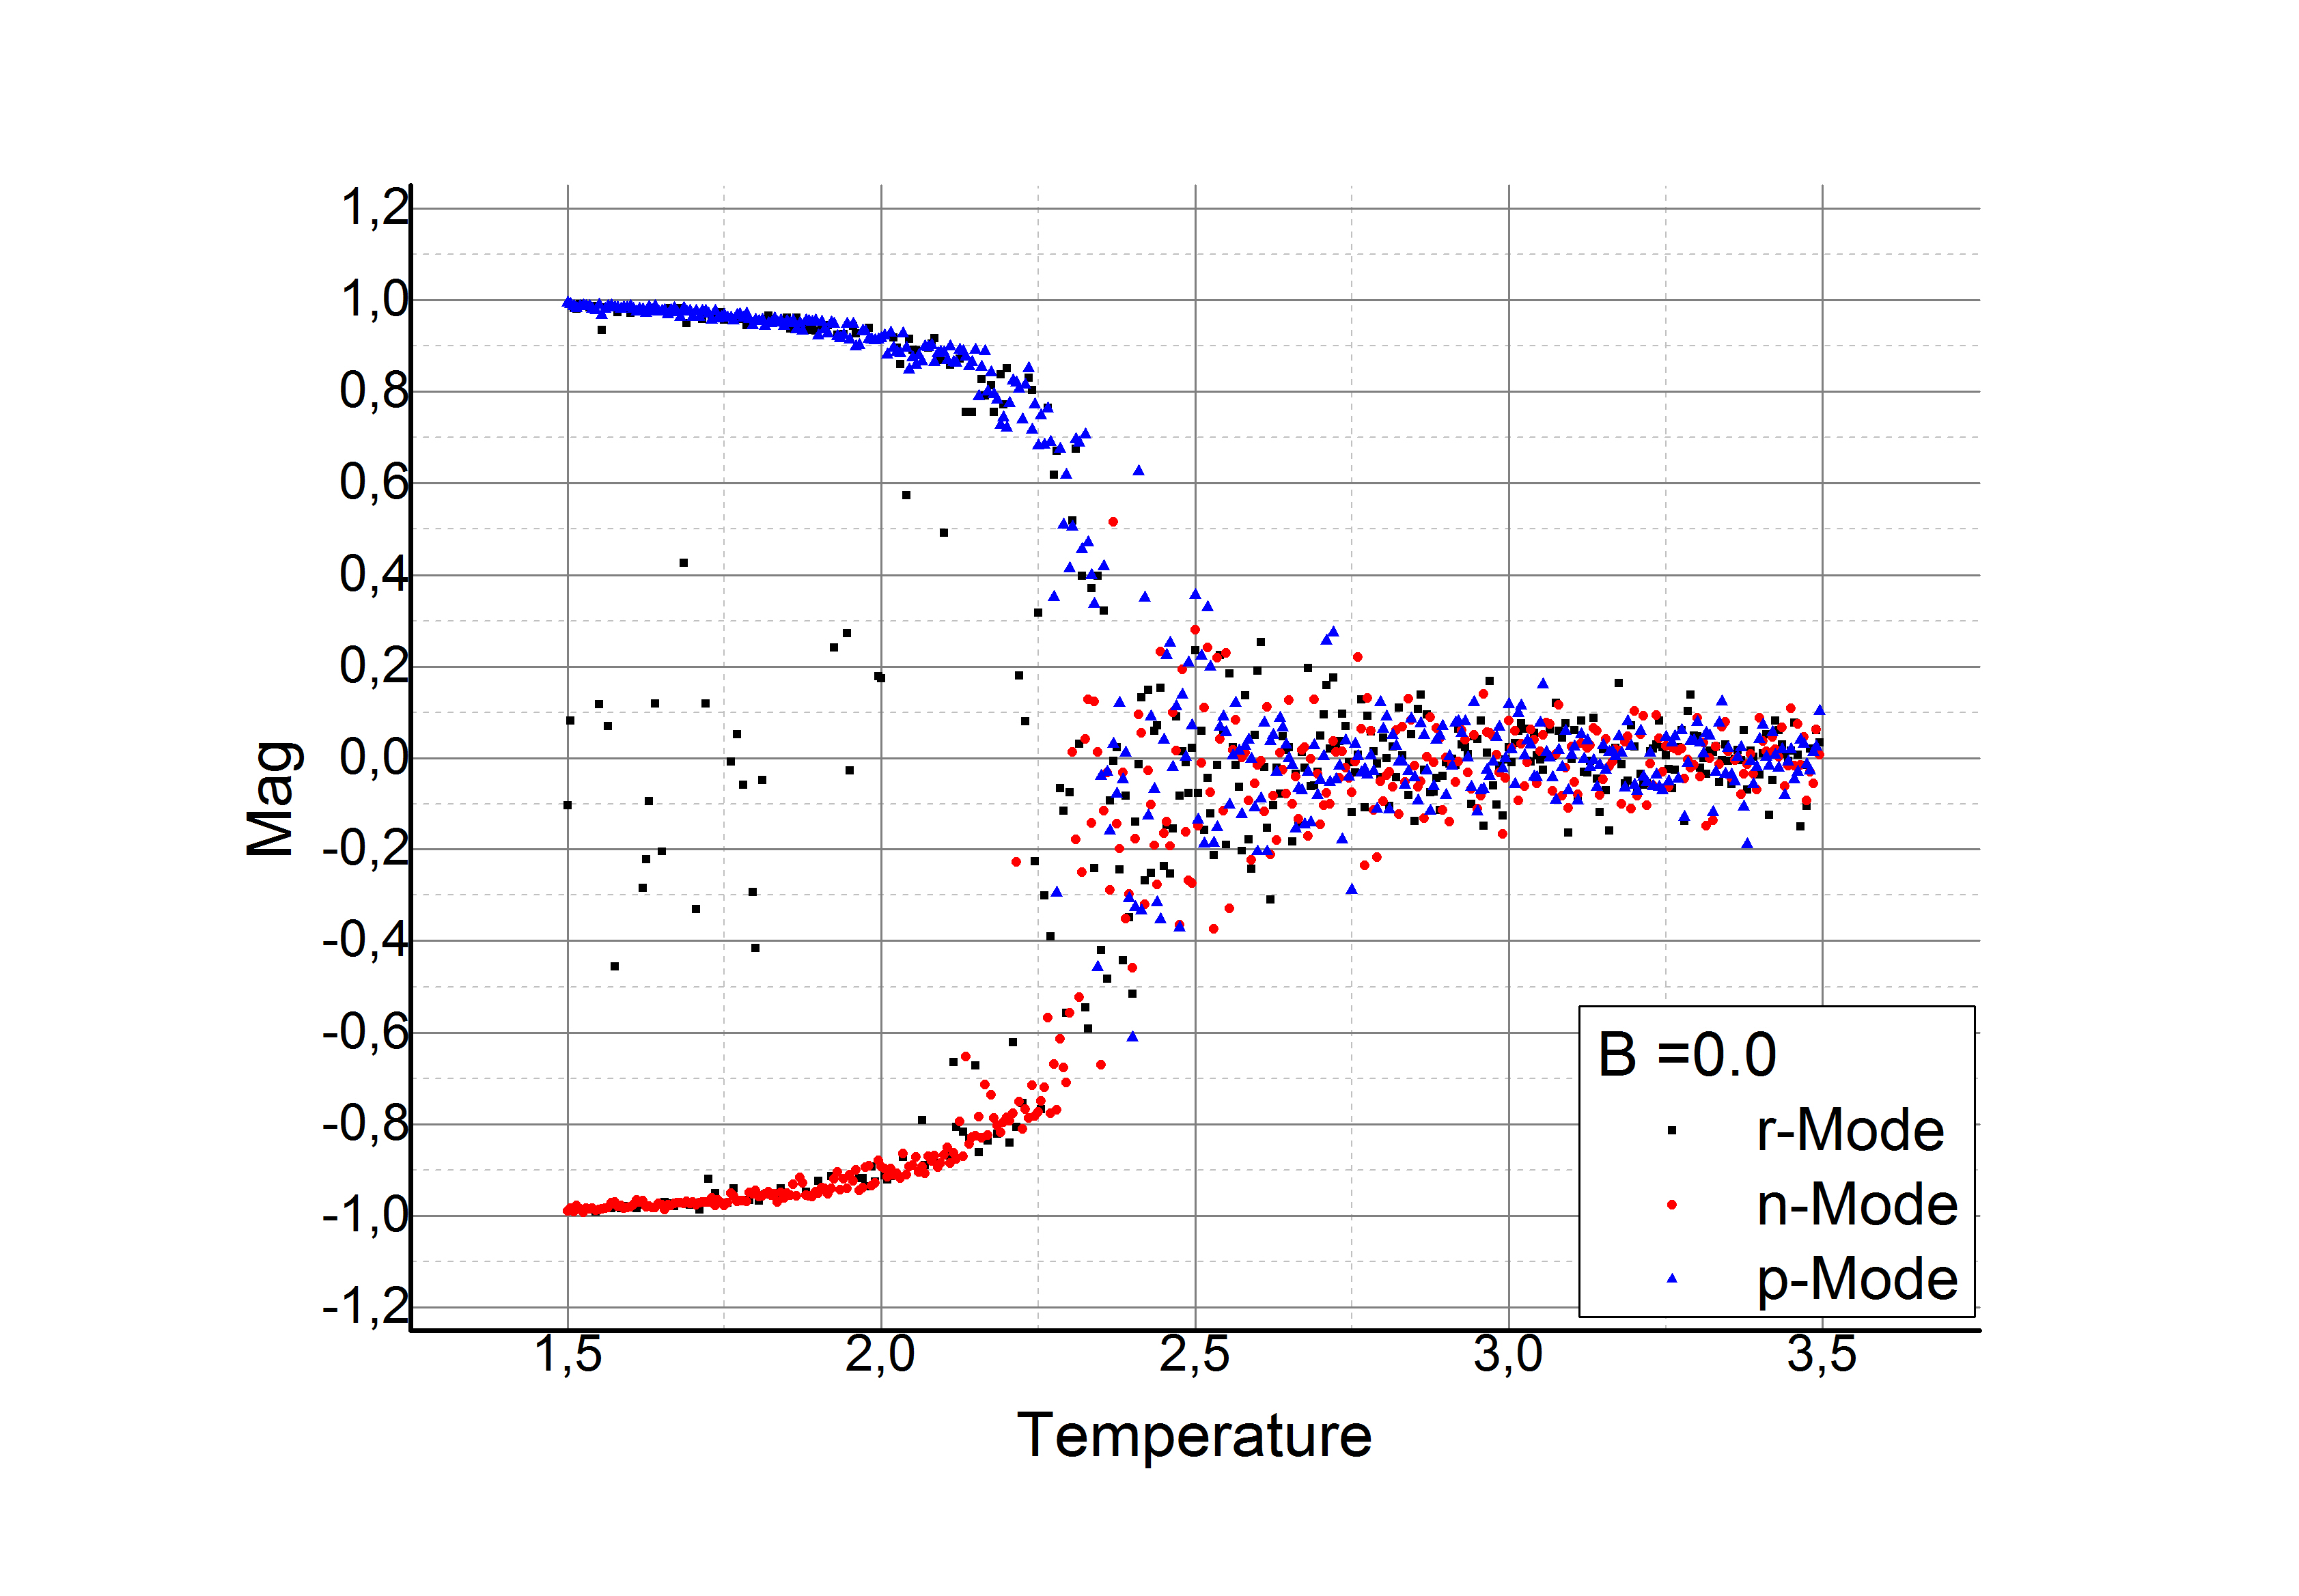
\includegraphics[width=0.47\textwidth]{../Graph_Export/MP2D/m(T)_B=0_matModes_MP2D_50_Plot.jpg}
	}		
	\caption{Temperaturabhängigkeit der Magnetisierung auf einem 50x50 Gitter}
	\label{}
\end{figure}

Die Temperaturabhängigkeit unterscheidet sich nur im Detail. So gibt es keine Ausreißer mehr, im Bereich zwischen 1.5 und 2.2. Zustände, die den lokalen Metropolis bisher verklemmt haben, werden durch den globalen Ansatz unschädlich gemacht. 
